\chapter{Theoretical Background}
\thispagestyle{empty}

Before discussing the experimental work, the theoretical foundations relevant to this thesis are introduced. The chapter begins with Gaussian beam optics and the beam quality factor \(M^2\), since these concepts are important for characterizing the laser sources used in the interferometer. Afterwards, the basic principle of interferometry is explained using a Michelson interferometer, which forms the basis of the measurement setup. This is then extended to quadrature homodyne interferometry, because this method also allows the direction of motion to be determined. The following sections introduce the main components of the experiment: suitable laser sources and the operating principle and limitations of the electronic translation stage.
\section{Gaussian Beam Optics}

One objective of this thesis was the characterization of different laser sources. In many optical applications, laser beams are assumed to be Gaussian, with a beam profile that follows the Gaussian distribution. For this reason, Gaussian beam optics forms the basis for one important characterization parameter, the beam quality factor \(M^2\). 

\subsection{Gaussian Beam}

Laser beams are solutions of Maxwell's equations, and the Gaussian beam represents a particular solution. To understand the origin of this solution, we first consider the wave equation for monochromatic electromagnetic fields. In this case, the spatial field distribution is governed by the Helmholtz equation

\begin{equation}
\nabla^2 \tilde{E} + k^2\tilde{E} = 0,
\end{equation}

where \(\tilde{E}\) is the complex field amplitude and \(k=2\pi/\lambda\) is the wave number \prismcite{7}.

In laser optics one is mainly interested in beams propagating predominantly along the \(z\)-direction with small transverse angles. Under this paraxial approximation the electric field can be separated into a rapidly oscillating carrier wave and a slowly varying complex envelope

\begin{equation}
\tilde{E}(x,y,z)=\tilde{u}(x,y,z)e^{-ikz}
\end{equation}
where \(\tilde{E}(x,y,z)\) is the complex electric field amplitude, \(\tilde{u}(x,y,z)\) is the slowly varying envelope, and \(e^{-ikz}\) represents the rapidly varying phase factor of propagation in the \(z\)-direction \prismcite{8}.



Substituting this expression into the Helmholtz equation and applying the paraxial approximation yields the paraxial Helmholtz equation

\begin{equation}
\nabla_T^2 \tilde{u}
- i\,2k \frac{\partial \tilde{u}}{\partial z}
=0,
\end{equation}

where \(\nabla_T^2\) is the transverse Laplace operator, \(i=\sqrt{-1}\) is the imaginary unit, and \(\partial/\partial z\) denotes the paraxial derivative with respect to the propagation direction \(z\). The quantities \(\tilde{u}\) and \(k\) are defined as before \prismcite{7}.

One solution of the paraxial Helmholtz equation is the paraboloidal wave

\begin{equation}
\tilde{u}(\rho,z)=\frac{A_1}{z}
\exp\left(-ik\frac{\rho^2}{2z}\right),
\end{equation}

where \(A_1\) is a constant complex amplitude, \(z\) is the propagation distance, and

\begin{equation}
\rho^2=x^2+y^2
\end{equation}

defines the radial coordinate in the transverse plane. Here, \(x\) and \(y\) are the transverse Cartesian coordinates \prismcite{7}.

Using the complex beam parameter

\begin{equation}
q(z)=z+iz_0,
\end{equation}

where \(z_0\) is the Rayleigh length, the Gaussian beam solution can be written as

\begin{equation}
\tilde{u}(\rho,z)=\frac{A_1}{q(z)}
\exp\left[-ik\frac{\rho^2}{2q(z)}\right]
\end{equation}

\prismcite{7}.

The complete complex electric field amplitude of a Gaussian beam is then given by

\begin{equation}
\tilde{E}(\rho,z)=A_0\frac{W_0}{W(z)}
\exp\left[-\frac{\rho^2}{W^2(z)}\right]
\exp\left[-ikz-ik\frac{\rho^2}{2R(z)}+i\zeta(z)\right],
\end{equation}

where \(A_0\) is the field amplitude at the beam waist, \(W_0\) is the beam waist radius, \(W(z)\) is the beam radius at the position \(z\), \(R(z)\) is the radius of curvature of the wavefront, and \(\zeta(z)\) is the Gouy phase shift \prismcite{7}.



\prismcite{9}.

Having established the field distribution of a Gaussian beam, the next step is to examine the parameters that characterize its propagation. In particular, the beam waist and beam divergence provide a quantitative description of the beam size and its evolution along the propagation direction.


\subsection{Beam Waist and Divergence}

The beam radius \(w(z)\) reaches its minimum value at the beam waist, which is located in the transverse plane defined by \(z=0\). The minimum beam radius at this position is denoted by \(w_0\) \prismcite{10}.

The propagation of the Gaussian beam radius along the \(z\)-direction is described by

\begin{equation}
w(z)=w_0\left[1+\left(\frac{z}{z_0}\right)^2\right]^{1/2}
\label{eq:beam_radius_propagation}
\end{equation}

where \(z_0\) is the Rayleigh range, defined as the distance from the beam waist at which the beam radius has increased by a factor of \(\sqrt{2}\) \prismcite{9}.

Far from the beam waist, the beam radius increases approximately linearly with the propagation distance, forming a divergence cone. The half-angle beam divergence is given by

\begin{equation}
\theta_0=\frac{\lambda}{\pi w_0},
\end{equation}

where \(\lambda\) is the wavelength of the laser beam and \(w_0\) is the beam waist radius \prismcite{10}.





The Gaussian beam described in the previous sections represents an idealized beam and provides the theoretical lower limit for beam divergence at a given beam waist. In practice, however, real laser beams often deviate from this ideal behavior. To quantify the extent of these deviations and compare the quality of different laser sources, the beam quality factor \(M^2\) is introduced.

\subsection{Beam Quality Factor}

Different resonator geometries support different transverse solutions of the wave equation and therefore different transverse laser modes. The fundamental transverse electromagnetic mode is the \(\mathrm{TEM}_{00}\) mode, which exhibits a Gaussian intensity distribution \prismcite{11}.
By shifting the waist position to \(z_0\) and denoting the Rayleigh range as \(z_R\), the propagation of the beam radius from Equation \eqref{eq:beam_radius_propagation} can be rewritten as

\begin{equation}
w^2(z)=w_0^2\left[1+\left(\frac{z-z_0}{z_R}\right)^2\right],
\end{equation}

where \(w_0\) is the beam waist radius, \(z_0\) the waist position and \(z_R\) the Rayleigh range \prismcite{12}.

For an ideal Gaussian beam, the intensity distribution is given by

\begin{equation}
I(r)=I_0\exp\left(-\frac{2r^2}{w^2}\right),
\end{equation}

where \(I(r)\) is the optical intensity at the radial distance \(r\) from the beam center, \(I_0\) is the peak intensity at the beam center \((r=0)\), and \(w\) is the beam radius, defined as the radius at which the intensity has decreased to \(1/e^2\) of its maximum value \prismcite{12}.

Anthony Siegman generalized this formalism for arbitrary real laser beams by introducing beam widths based on the statistical standard deviation of the intensity distribution:

\begin{equation}
w_x(z)=2\sigma_x(z),
\end{equation}

where \(w_x(z)\) is the beam radius in the \(x\)-direction at the propagation distance \(z\), and \(\sigma_x(z)\) is the standard deviation of the intensity distribution in the \(x\)-direction \prismcite{12}.

The propagation of real, non-ideal laser beams can then be described by the \(M^2\)-formalism:

\begin{equation}
w_x^2(z)=w_{0x}^2+
M_x^4\left(\frac{\lambda}{\pi w_{0x}}\right)^2(z-z_{0x})^2,
\end{equation}

where \(w_x(z)\) is the beam radius in the \(x\)-direction at the propagation distance \(z\), \(w_{0x}\) is the minimum beam radius (beam waist) in the \(x\)-direction, \(M_x^2\) is the beam quality factor in the \(x\)-direction, \(z_{0x}\) is the position of the beam waist, and \(\lambda\) is the wavelength of the laser beam \prismcite{12}.

The beam quality factor satisfies

\begin{equation}
M^2 \ge 1,
\end{equation}

where \(M^2=1\) corresponds to an ideal diffraction-limited Gaussian beam, while larger values indicate reduced beam quality due to higher-order modes or optical distortions \prismcite{12}.

The divergence of a real beam is therefore given by

\begin{equation}
\theta = M^2\frac{\lambda}{\pi w_0},
\end{equation}

where \(\theta\) is the far-field divergence half-angle, \(M^2\) is the beam quality factor, \(w_0\) is the beam waist radius, and \(\lambda\) is the wavelength of the laser beam. This equation shows that beams with \(M^2>1\) diverge more strongly than an ideal Gaussian beam \prismcite{12}.

The beam quality factor \(M^2\) therefore provides an important criterion for evaluating laser sources. 

After the basic properties of laser beams have been introduced, the next step is to describe how such beams can be used for displacement measurements. For this reason, the following section explains the principle of interferometry.

\section{Systems for Interferometry}

\subsection{Michelson Interferometer}

The Michelson interferometer is one of the most important interferometric setups in optics and precision metrology. A Michelson interferometer consists of a beam splitter and two mirrors. A coherent light beam enters the interferometer and a beam splitter divides it into two beams of identical intensity that travel along different optical paths. After being reflected by the mirrors, the beams recombine \prismcite{2}. The setup is shown in Figure~\ref{fig:michelsoninterferometer}.

\begin{figure}[htbp]
    \centering
    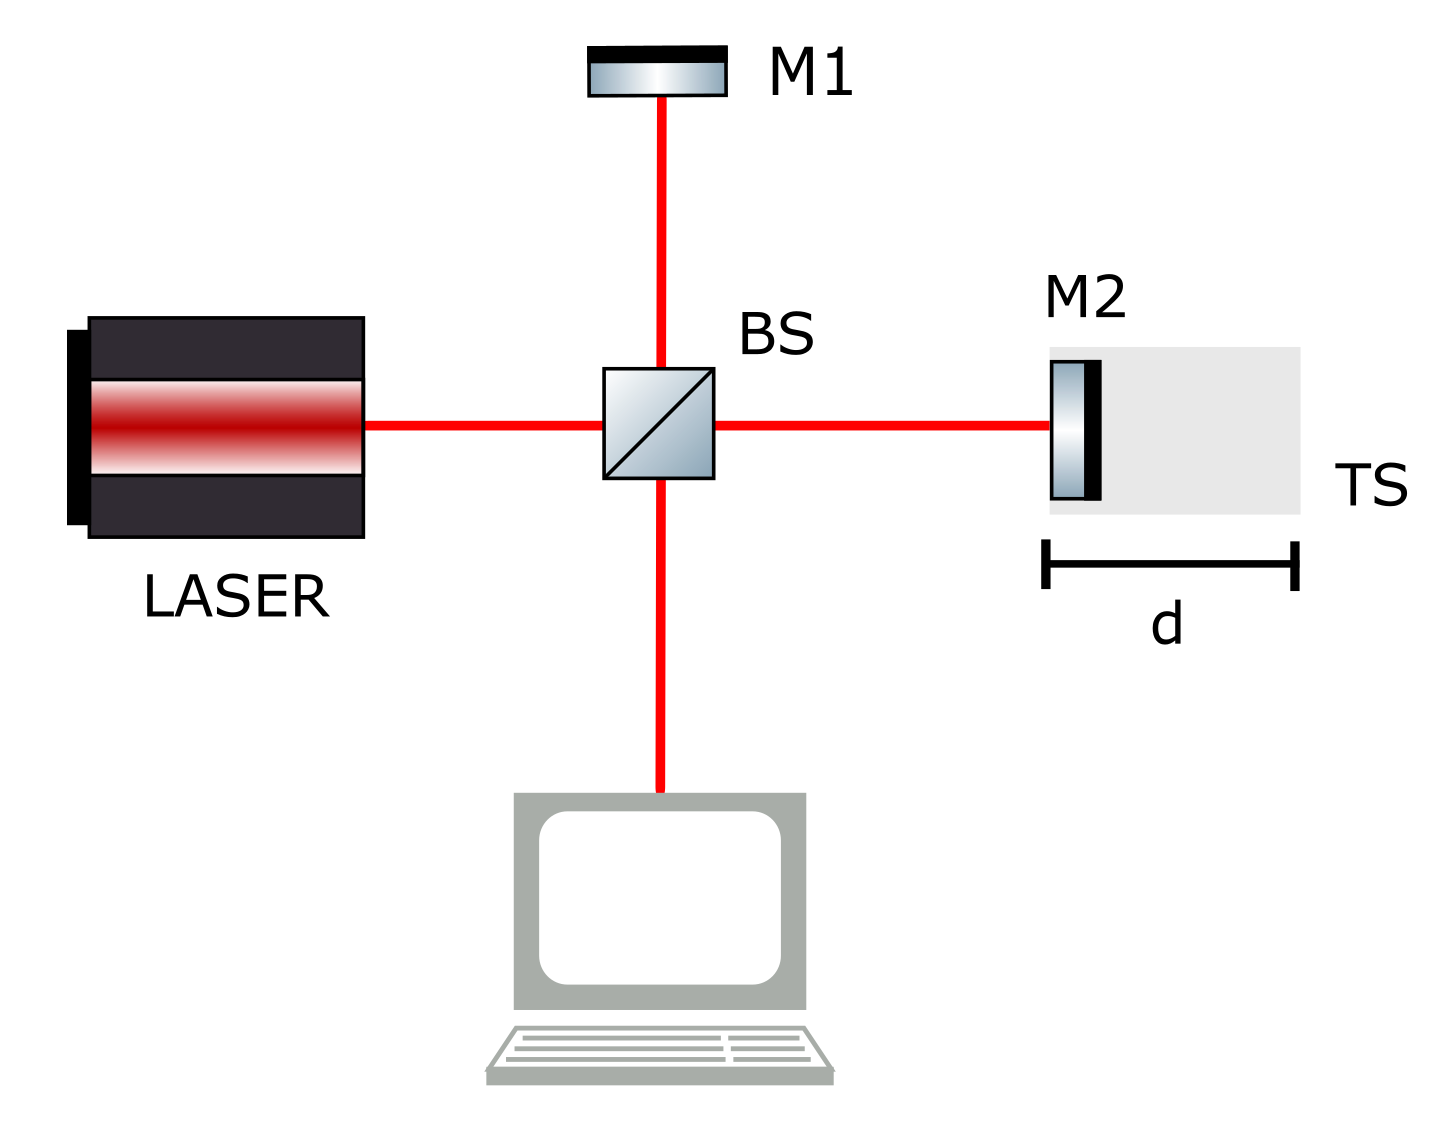
\includegraphics[width=0.55\linewidth]{figures/michelsongeneral.png}
    \caption{Schematic representation of a Michelson interferometer. The incoming beam is split at the beam splitter, denoted by BS, into two beams that propagate along the two interferometer arms. After reflection at mirrors M1 and M2, the beams recombine at the beam splitter and their interference can be detected. The mirror M2 creates an optical path difference by moving a distance d on a Translation Stage TS.}
    \label{fig:michelsoninterferometer}
\end{figure}

The electric field of the incoming plane wave can be written as
\begin{equation}
E_l = A_l \cos(\omega t-kz),
\end{equation}
where \(A_l\) is the field amplitude, \(\omega\) is the angular frequency, \(t\) is the time, \(k\) is the wave number, and \(z\) is the propagation coordinate \prismcite{2}.

The electric fields of the two partial waves \(E_1\) and \(E_2\) after propagation through the interferometer are given by
\begin{equation}
E_1 = \sqrt{RT}A_l\cos(\omega t+\varphi_1)
\end{equation}
and
\begin{equation}
E_2 = \sqrt{RT}A_l\cos(\omega t+\varphi_2),
\end{equation}
where \(R\) and \(T\) denote the intensity reflection and transmission coefficients of the beam splitter, and \(\varphi_1\) and \(\varphi_2\) are the optical phases accumulated in the two interferometer arms \prismcite{2}.

The detected instantaneous intensity results from the superposition of the two electric fields:
\begin{equation}
\begin{aligned}
I_T &= c\varepsilon_0(E_1+E_2)^2 \\
    &= c\varepsilon_0 RT A_l^2 \left[ \cos(\omega t+\varphi_1) + \cos(\omega t+\varphi_2) \right]^2,
\end{aligned}
\label{eq:instantaneous_intensity}
\end{equation}
where \(c\) is the speed of light and \(\varepsilon_0\) is the vacuum permittivity \prismcite{2}.

Since the detector averages over many optical periods, the time-averaged intensity \(\bar{I}_T = \langle I_T \rangle\) is measured. Using the trigonometric identity for the sum of cosines and taking the time average of Eq.~\eqref{eq:instantaneous_intensity} yields
\begin{equation}
\bar{I}_T = c\varepsilon_0 RT A_l^2 (1 + \cos\Delta\varphi).
\end{equation}
By defining the time-averaged intensity of the incident laser beam as
\begin{equation}
I_0 = \frac{1}{2}c\varepsilon_0 A_l^2,
\end{equation}
the final expression for the detected time-averaged intensity becomes
\begin{equation}
\bar{I}_T = 2RTI_0(1+\cos\Delta\varphi),
\label{eq:time_averaged_intensity}
\end{equation}
with the phase difference
\begin{equation}
\Delta\varphi = \varphi_1-\varphi_2=\frac{2\pi}{\lambda}\Delta s,
\label{eq:phase_difference}
\end{equation}
where \(\Delta s\) is the optical path difference between the two interferometer arms and \(\Delta\varphi\) is the phase difference \prismcite{5}.



\subsubsection{Interference}
Interference describes the superposition of coherent electromagnetic waves. As already noted in Eq.~(\ref{eq:phase_difference}), the optical path difference determines the phase difference between the two interfering waves. Constructive interference occurs when the optical path difference is an integer multiple of the wavelength,
\begin{equation}
\Delta s = m\lambda,
\end{equation}
which corresponds to a phase difference of
\begin{equation}
\Delta\varphi = 2\pi m,
\end{equation}
where \(m\in\mathbb{Z}\). Conversely, destructive interference occurs for optical path differences of
\begin{equation}
\Delta s = \left(m+\frac{1}{2}\right)\lambda,
\end{equation}
corresponding to a phase difference of
\begin{equation}
\Delta\varphi = (2m+1)\pi.
\end{equation} Therefore, very small displacements can be detected by counting interference fringes \prismcite{6}.




\subsubsection{Fringe Counting}

The Michelson interferometer was chosen because it is a simple and well-established configuration for displacement measurements. One method of evaluating the interference signal from it is fringe counting. Since this method is applied in this work, it is briefly introduced in the following.

In the Michelson Interferometer, the movement of one mirror changes the optical path difference between the two interferometer arms. Whenever the optical path difference changes by one wavelength, one complete interference fringe passes the detector.

For a Michelson interferometer the stage displacement \(d\) of the moving mirror is related to the number of counted fringes \(N\) by

\begin{equation}
d = \frac{N\lambda}{2}
\end{equation}

\prismcite{5}.

\subsection{Quadrature Homodyne Interferometry}

A conventional Michelson interferometer like explained above is a homodyne interferometer, meaning that both interfering beams originate from the same laser source and therefore possess the same optical frequency. \prismcite{29}

While a conventional homodyne interferometer can measure displacement with high precision, it cannot determine the direction of motion. This limitation arises because the detected intensity depends on the cosine of the phase difference, which is an even function:

\begin{equation}
\cos(\Delta\varphi)=\cos(-\Delta\varphi).
\end{equation}

As a result, identical intensity values are obtained for positive and negative displacements, making it impossible to distinguish whether the translation stage is moving forward or backward \prismcite{30}.

To overcome this ambiguity, quadrature homodyne interferometry has been developed. In this technique, two interference signals with a phase offset of $90^\circ$ are generated. The resulting detector signals can be written as

\begin{equation}
S_1=A\cos(\Delta\varphi),
\end{equation}

and

\begin{equation}
S_2=A\sin(\Delta\varphi),
\end{equation}

where $A$ is the signal amplitude. These signals are commonly referred to as quadrature signals because they are shifted by one quarter of a period relative to each other \prismcite{30}.
In the setup (as shown in Figure~\ref{fig:homodyne_setup}), the simultaneous detection of the s- and p-polarized components provides directional information about the phase shift. In contrast, a conventional interferometer typically measures only one polarization component, making it difficult to distinguish the sign of the phase change.

\begin{figure}[H]
    \centering
    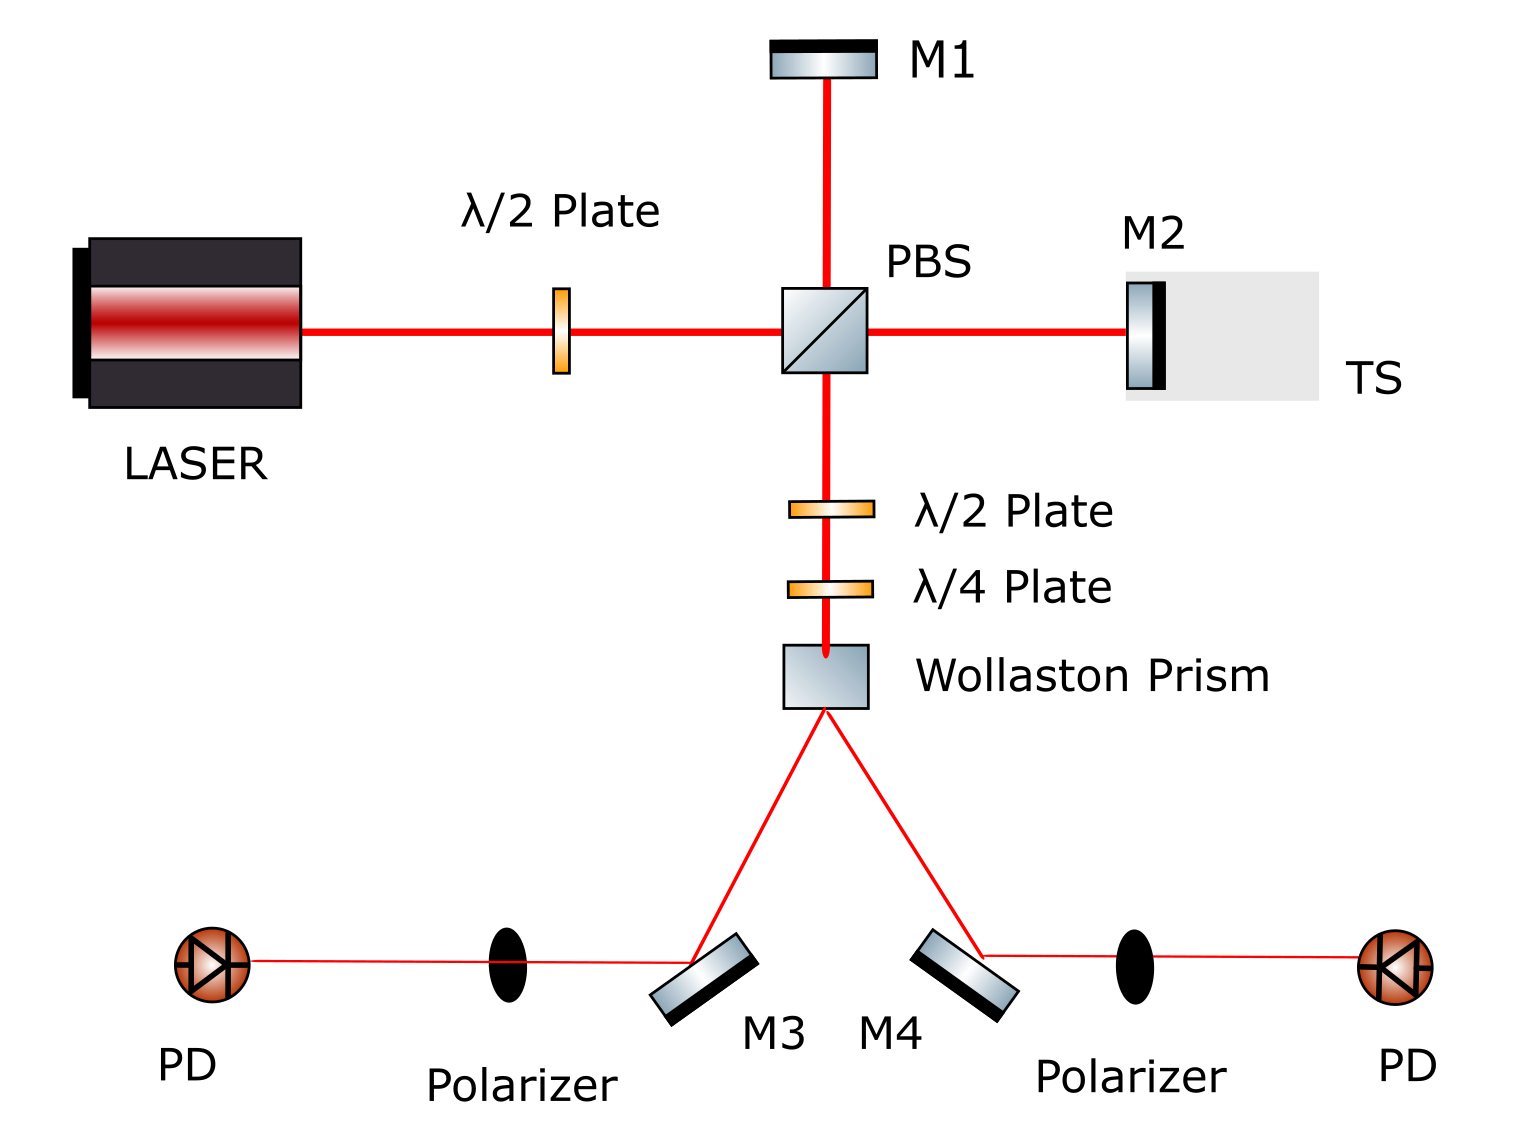
\includegraphics[width=0.55\linewidth]{figures/homodyneschematic.png}
    \caption{Setup for quadrature homodyne interferometry. This configuration visualizes the principle of quadrature signal generation. PBS denotes a polarizing beam splitter, BS describes a beam splitter, M1 -- M4 Mirrors, PD a photodiode.}
    \label{fig:homodyne_setup}
\end{figure}


The two signals can be represented as coordinates in the $(S_1,S_2)$ plane (as shown in Figure~\ref{fig:counting_homodyne}). Ideally, the resulting trajectory forms a circle as the stage moves. The phase can then be reconstructed continuously using

\begin{equation}
\Delta\varphi=\operatorname{atan2}(S_2,S_1),
\end{equation}

which uniquely determines the phase over the full $2\pi$ range \prismcite{31}.

\begin{figure}[htbp]
    \centering
    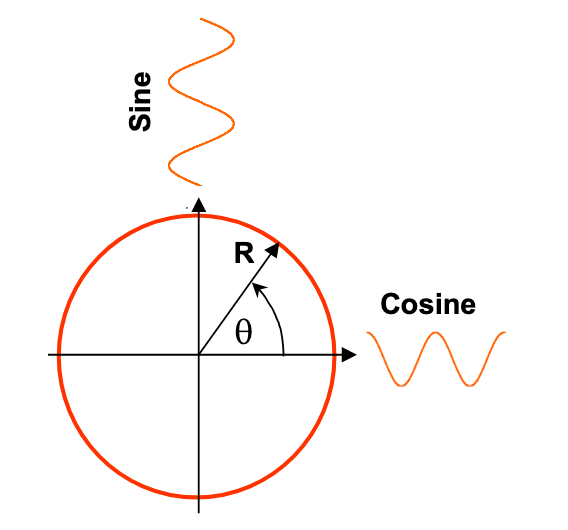
\includegraphics[width=0.55\linewidth]{figures/countinghomodyne.png}
    \caption{Principle of direction-sensitive quadrature signal evaluation in homodyne interferometry. The phase relation between two quadrature signals enables the direction of motion to be determined. Obtained from \prismcite{31}.}
    \label{fig:counting_homodyne}
\end{figure}

Unlike a conventional homodyne interferometer, the direction of motion can now be determined from the temporal evolution of the reconstructed phase. As the translation stage moves in the positive direction, the phase increases continuously. Conversely, motion in the opposite direction causes the phase to decrease \prismcite{30}. The direction is therefore obtained from the sign of the phase change between consecutive measurements,

\begin{equation}
\frac{d\Delta\varphi}{dt}>0
\quad \Rightarrow \quad
\text{forward motion},
\end{equation}

\begin{equation}
\frac{d\Delta\varphi}{dt}<0
\quad \Rightarrow \quad
\text{backward motion}.
\end{equation}

This can also be interpreted geometrically. In the $(S_1,S_2)$ plane, positive motion causes the measured signal vector to rotate counterclockwise, whereas negative motion results in clockwise rotation. By tracking the phase continuously, both displacement and direction can therefore be determined unambiguously.

The displacement is obtained from the measured phase according to

\begin{equation}
d= \frac{\lambda}{4\pi}\Delta\varphi,
\end{equation}

where \(d\) is the displacement of the moving mirror on the translation stage, \(\lambda\) is the laser wavelength, and \(\Delta\varphi\) is the measured phase change \prismcite{32}.

Since the phase can be tracked continuously, quadrature homodyne interferometry can measure displacements much smaller than the laser wavelength \prismcite{33}. It also provides information about the direction of movement, making it possible to track the position reliably over long distances. For these reasons, a quadrature homodyne interferometer was chosen as an extension for the displacement measurement system developed in this thesis.

To realize the expanded capabilities of quadrature homodyne interferometry compared to a conventional Michelson interferometer, additional optical elements are required. Specifically, polarization-controlling components are essential for generating the quadrature signals. These components and their operating principles are introduced in the following.

\subsubsection{Optical Components for Quadrature Homodyne Interferometry}

For completeness, the most important optical components used in the quadrature homodyne interferometer are briefly introduced.
Specifically, a $\lambda/2$ wave plate, a $\lambda/4$ wave plate and a Wollaston prism. The basic functions of a conventional beam splitter and a polarizing beam splitter are only mentioned briefly here. A conventional beam splitter divides the incoming beam into two beams of similar intensity, while a polarizing beam splitter separates the beam into two orthogonal polarization components. The Wollaston prism is discussed in more detail because it is a special type of polarizing beam splitter.

\paragraph{Half-Wave Plate}

A half-wave plate is a special type of wave retarder. In general, a wave retarder is a birefringent optical element with two principal axes, usually referred to as the fast and slow axes. Because the refractive indices along these axes are different, the two orthogonal polarization components of a beam propagate with different phase velocities. As a result, a phase delay is introduced between the two components \prismcite{34}.

For a half-wave plate, this phase retardance is

\begin{equation}
    \Gamma = \pi .
\end{equation}

This means that one polarization component is delayed by half an optical period with respect to the orthogonal component. For linearly polarized input light, the output remains linearly polarized, but the plane of polarization is rotated. If the incident polarization forms an angle \(\theta\) with one of the principal axes of the half-wave plate, the polarization direction after the plate is rotated by \(2\theta\) with respect to the incident direction \prismcite{35}.

In the quadrature homodyne interferometer, this property is used to adjust the polarization angle of the laser beam. By rotating the polarization to \(45^\circ\) with respect to the axes of a polarizing beam splitter, the optical power can be divided into two equal polarization components. 
\paragraph{Quarter-Wave Plate}
A quarter-wave plate operates in the same way as a half-wave plate but introduces a phase retardance of

\begin{equation}
\Gamma=\frac{\pi}{2}.
\end{equation}

Consequently, one polarization component is delayed by one quarter of an optical period relative to the orthogonal component. If linearly polarized light is incident at an angle of \(45^\circ\) to the principal axes, the output becomes circularly polarized. Conversely, circularly polarized light is converted into linearly polarized light \prismcite{35}.

\paragraph{Wollaston Prism}

A Wollaston prism, shown in Figure~\ref{fig:wollaston_prism}, is a polarization beam splitter that separates an incoming beam into two linearly polarized output beams. It consists of two birefringent wedge prisms, commonly made from a material such as calcite. Although a magnesium fluoride (\(\mathrm{MgF}_2\)) Wollaston prism was used in this work due to availability, this choice of material does not affect the operating principle. The two wedges are joined together with their optical axes oriented perpendicular to each other \prismcite{36}. Because birefringent materials exhibit different refractive indices for different polarization directions, the ordinary and extraordinary polarization components experience different refraction angles. The behavior, that different refractive indices are refracted differently originates from Snell's law,
\begin{equation}
    n_1 \sin\theta_1 = n_2 \sin\theta_2,
\end{equation}
where \(n_1\) and \(n_2\) are the refractive indices of the first and second medium, respectively, and \(\theta_1\) and \(\theta_2\) are the angles of incidence and refraction, measured with respect to the surface normal \prismcite{37}.

In the first prism, one polarization component propagates as the ordinary ray while the orthogonal component propagates as the extraordinary ray. In the second prism, whose optical axis is rotated by \(90^\circ\), these roles are interchanged. As a result, the two polarization components are refracted in opposite directions at the internal interface and leave the prism as two spatially separated beams. The use of two prisms increases the angular separation and makes the two output beams easier to use experimentally.

\begin{figure}[htbp]
    \centering
    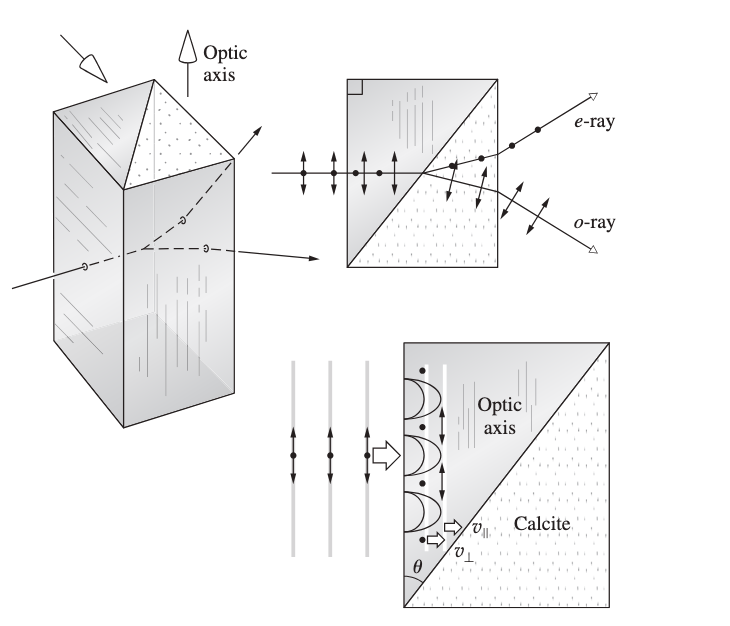
\includegraphics[width=0.55\linewidth]{figures/wollaston.png}
    \caption{Schematic representation of a Wollaston prism. The two cemented birefringent prisms have perpendicular optical axes, causing orthogonally polarized components to be refracted in different directions. Obtained from \prismcite{36}.}
    \label{fig:wollaston_prism}
\end{figure}


After introducing the different interferometric configurations, the next step is to consider how such a setup can be realized experimentally. One of the most important components is the laser source. Since different laser technologies have different advantages and limitations, the following section introduces two laser types that are especially relevant for interferometric applications.

\section{Laser Sources for Interferometry}

Traditionally, helium-neon (HeNe) lasers are widely used in interferometry \prismcite{13}. Semiconductor diode lasers, however, have become increasingly attractive due to their compact design and high efficiency \prismcite{14}.

In this work, several HeNe lasers and one semiconductor diode laser were investigated as potential laser sources for the interferometric calibration system. The following sections summarize the operating principles and characteristic properties of both laser types.
\subsection{Helium-Neon (HeNe) Lasers}

The Helium-Neon (HeNe) laser is one of the most widely used gas lasers in optics and interferometry. HeNe lasers emit coherent red light at a wavelength of \(632.8\,\mathrm{nm}\) and operate in continuous-wave mode \prismcite{15}. The emitted laser beam exhibits a narrow spectral bandwidth, high temporal and spatial coherence as well as low beam divergence. \prismcite{15}. High coherence is essential because stable interference fringes can only be observed if the phase relation between the interfering waves remains constant over time \prismcite{17}. Due to these properties, HeNe lasers are particularly suitable for interferometric measurements and precision optical experiments \prismcite{15}.



\subsubsection{Operating Principle}

A schematic setup of a typical HeNe laser is shown in Figure~\ref{fig:hene_setup}. The laser consists of a gas discharge tube filled with a mixture of helium and neon gas \prismcite{18}.

\begin{figure}[H]
    \centering
    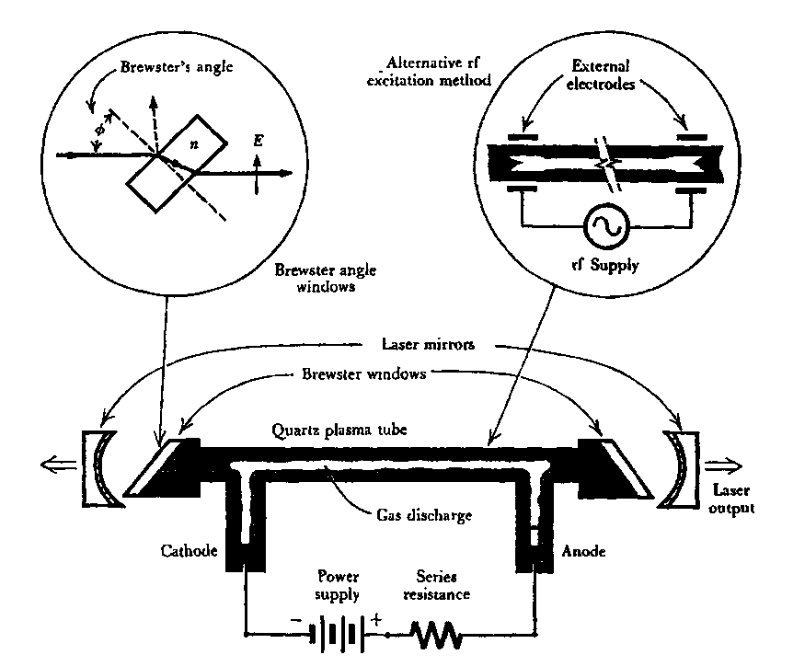
\includegraphics[width=0.55\linewidth]{figures/HeNeLaserAufbau.png}
    \caption{Schematic setup of a HeNe laser (obtained from \prismcite{19}).}
    \label{fig:hene_setup}
\end{figure}

The laser process in a HeNe laser begins with an electrical gas discharge inside a mixture of helium and neon gas. A short high-voltage pulse excites free electrons within the discharge tube. These electrons collide predominantly with helium atoms and excite them into metastable energy states \prismcite{20}.

The energies of the metastable helium states match specific excited energy levels of neon atoms. During collisions between helium and neon atoms, the excitation energy can therefore be transferred efficiently from helium to neon. As a consequence, neon atoms are excited into higher energy states without requiring direct excitation \prismcite{20}.

The continuous transfer of energy from helium to neon leads to the formation of a population inversion in the neon atoms. In this condition, more neon atoms occupy excited states than lower-energy states, which is a necessary requirement for laser amplification. Neon therefore forms the active gain medium of the laser, whereas helium mainly serves as the pumping medium that enables the excitation process \prismcite{20}.

Figure~\ref{fig:hene_levels} illustrates the simplified energy level scheme of the HeNe laser.

\begin{figure}[H]
    \centering
    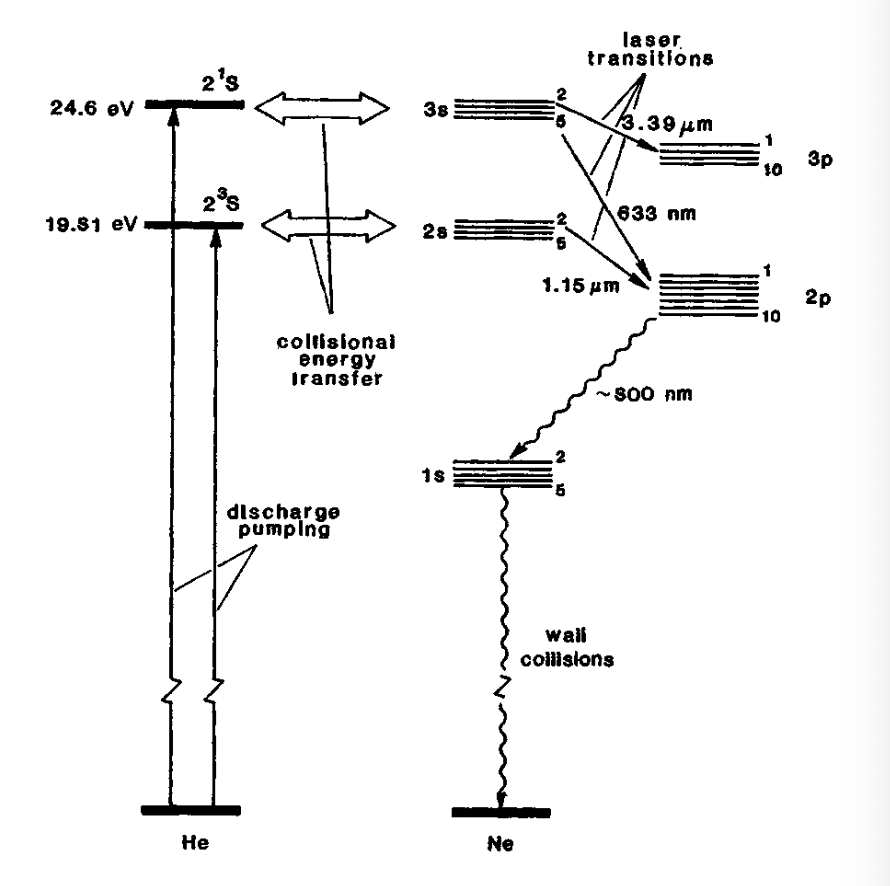
\includegraphics[width=0.55\linewidth]{figures/HeNeLaserEnergyLevels.png}
    \caption{Simplified energy level diagram of the HeNe laser (obtained from \prismcite{21}).}
    \label{fig:hene_levels}
\end{figure}

Laser emission occurs through stimulated emission in neon atoms. Excited neon atoms transition from the upper laser level to a lower energy level and emit photons with a wavelength of \(632.8\,\mathrm{nm}\). These photons are reflected repeatedly between two mirrors forming the optical resonator. One mirror has a very high reflectivity, while the second mirror is partially transmitting. The repeated reflections amplify the optical field inside the resonator, and a fraction of the amplified radiation exits through the partially transmitting mirror as the visible laser beam \prismcite{20}.

\subsection{Semiconductor Diode Lasers}

Semiconductor diode lasers are compact and efficient laser sources. In contrast to gas lasers such as HeNe lasers, laser generation in diode lasers is based on charge carrier recombination inside a semiconductor pn-junction \prismcite{22}.

Diode lasers offer several practical advantages including compact size, low electrical power consumption, high efficiency, and comparatively low manufacturing costs \prismcite{14}.

\subsubsection{Operating Principle}

A semiconductor diode laser (as shown in Figure~\ref{fig:semiconductor_laser_structure}) consists of two differently doped semiconductor regions forming a pn-junction. One semiconductor region contains an excess of electrons and is referred to as the n-type material, while the other region contains an excess of holes and is referred to as the p-type material \prismcite{14}.

When a forward bias voltage is applied across the pn-junction, electrons from the n-type region and holes from the p-type region are injected into the junction region \prismcite{22}. In this active region, electrons and holes recombine and release energy in the form of photons \prismcite{14}.

The emitted photons stimulate further recombination events, resulting in stimulated emission. The resonator is typically formed by partially reflective semiconductor surfaces located at both ends of the laser chip \prismcite{14}.

\begin{figure}[H]
    \centering
    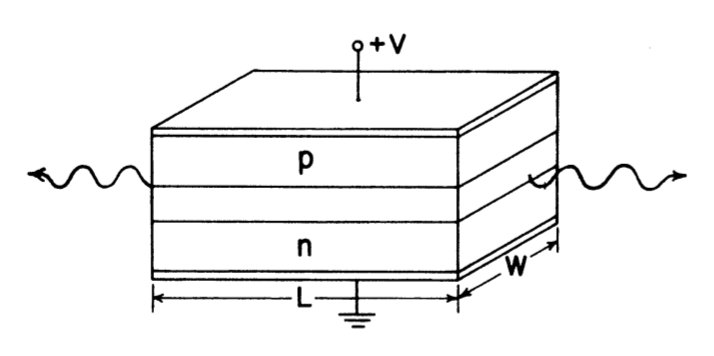
\includegraphics[width=0.55\linewidth]{figures/SemiconLaserStrucSimple.png}
    \caption{Schematic structure of a semiconductor diode laser. The active region is located at the pn-junction, where injected electrons and holes recombine and generate optical radiation. Obtained from \prismcite{16}}
    \label{fig:semiconductor_laser_structure}
\end{figure}

Compared to HeNe lasers, diode lasers often exhibit larger beam divergence \prismcite{23} and stronger temperature dependence \prismcite{24}. However, their compactness, efficiency, and practical stability characteristics make them attractive candidates for interferometric measurement systems \prismcite{25}.

After introducing the laser sources, the translation stage used in the experimental setup must also be considered. Since the interferometer is designed to measure and improve the positioning accuracy of the stage, its operating principle and limitations are discussed in the following.

\section{Motorized Translation Stage}

A motorized precision translation stage is used in the interferometer setup to generate controlled linear displacements of the mirror.

\subsection{Operating Principle}

Although the following description is based on the Physik Instrumente (PI) translation stage, the temporarily used Thorlabs stage operates according to the same fundamental principle: Linear motion is generated by converting the rotational motion of an electric motor into translational motion using a lead screw. The moving platform is guided by rolling-element linear bearings, which provide smooth motion with high stiffness and low friction. \prismcite{26, 27}

Although motorized translation stages provide highly repeatable and accurate positioning over long travel distances, their performance is inherently limited by both mechanical and environmental influences. These effects prevent the commanded position from exactly matching the actual position of the moving platform. The positioning accuracy is affected by mechanical tolerances, such as lead screw errors and bearing imperfections, as well as by thermal effects. Temperature variations cause thermal expansion of structural components, guide rails, and the drive mechanism, resulting in positioning errors, particularly over long travel distances. \prismcite{28}

Due to these mechanical and thermal limitations, the commanded stage position cannot be assumed to represent the true displacement of the mirror with nanometer accuracy. Therefore, an independent interferometric measurement system is used in this work to determine the actual displacement with higher precision.
